% !TEX root = ./main.tex
\graphicspath{{figures_manufactured/}}% Set graphics path location


\subsection{Method of Manufactured Solutions}

This section describes the test of HiFiLES's spatial order of accuracy using the Method of Manufactured Solutions (MMS) in 2D and 3D for viscous flows. As shown by Salari et. al\cite{salari2000code}, the MMS test rigorously assesses the correctness of implementation of a solver of Partial Differential Equations. We perform the MMS test in grids using simplex elements, as these are crucial for simulations in unstructured meshes and have a more complex implementation than squares and hexahedra.

The MMS test for NS solvers requires checking the solver's solution against an exact solution. Such an exact solution can be chosen arbitrarily. The NS equations can be satisfied with this arbitrary solution by including a time-dependent source term in the equations. Then, we solve

\begin{equation}
\frac{\partial U}{\partial t} +  \nabla \cdot {\bf F} = S
\end{equation}

For the following tests, we selected a smooth exact solution, so aliasing does not pollute the results. We picked

\begin{equation}\label{eq:NSwithSource}
U_{2D} = \l(
\begin{tabular}{c}
$\sin{(k(x+y) - \omega t)} + a$\\
$\sin{(k(x+y) - \omega t)} + a$\\
$\sin{(k(x+y) - \omega t)} + a$\\
$(\sin{(k(x+y) - \omega t)} + a)^2$
\end{tabular}
\r) \;\; 
U_{3D} = \l(
\begin{tabular}{c}
$\sin{(k(x+y+z) - \omega t)} + a$\\
$\sin{(k(x+y+z) - \omega t)} + a$\\
$\sin{(k(x+y+z) - \omega t)} + a$\\
$\sin{(k(x+y+z) - \omega t)} + a$\\
$(\sin{(k(x+y+z) - \omega t)} + a)^2$
\end{tabular}
\r)
\end{equation}

To find the value of $S$, we plug the values of our selected $U$ into the left-hand side of Equation~\eqref{eq:NSwithSource} and simplify. The resulting expression is $S$. 
We let Pr$=0.72, \gamma = 1.4, k = \pi, \omega = \pi, a = 3.0$ and $\mu = 0.001$.

The meshes used have dimensions $[-1,1] \times [-1,1]$ in 2D and $[-1,1] \times [-1,1] \times [-1,1]$ in 3D. Periodic boundary conditions were applied on the boundaries of the square and cube domains. Uniform square and cubic meshes were created and then each element was subdivided into triangles or tetrahedra. Two triangles were created from each square, and six tetrahedra were created from each cube. Consequently, in 2D a $N \times N$ mesh contains $2N^2$ triangles, and in 3D a $N \times N \times N$ mesh contains $6N^3$ tetrahedra. 


In 3D, the time step was $1$e$-4$ seconds and 10 seconds of flow were simulated. In 2D, the time step was $1$e$-6$ seconds and 1 second of flow was simulated. The time-stepping scheme used was the low-storage, $4^\text{th}$ order accurate RK45 method\cite{carpenter1994fourth}. 


\begin{table}[h]
\centering
\begin{tabular}{ c c c c c c c} 
  
 Mesh: &   & 2x2x2 & 4x4x4 & 8x8x8 & 16x16x16 & Overall Order \\ 
 \hline 
 \multirow{2}{*}{$p = 1$} & $L_2$ error & 5.76e-01 & 1.35e-01 & 3.22e-02 & 7.90e-03 &   \\ 
  
   & $\mathcal{O}(L_2)$ &   & 2.10 & 2.06 & 2.03 & 2.06 \\ 
 \hline 
 \multirow{2}{*}{$p = 2$} & $L_2$ error & 4.09e-01 & 5.52e-02 & 6.87e-03 & 8.53e-04 &   \\ 
  
   & $\mathcal{O}(L_2)$ &   & 2.89 & 3.01 & 3.01 & 2.97 \\ 
 \hline 
 \multirow{2}{*}{$p = 3$} & $L_2$ error & 9.77e-02 & 5.97e-03 & 3.78e-04 &   &   \\ 
  
   & $\mathcal{O}(L_2)$ &   & 4.03 & 3.98 &   & 4.01 \\ 
 \hline 
 \multirow{2}{*}{$p = 4$} & $L_2$ error & 1.12e-02 & 6.39e-04 & 2.07e-05 &   &   \\ 
  
   & $\mathcal{O}(L_2)$ &   & 4.13 & 4.95 &   & 4.54 \\ 
 \hline 
 \multirow{2}{*}{$p = 5$} & $L_2$ error & 1.53e-01 & 5.08e-03 & 6.92e-05 &   &   \\ 
  
   & $\mathcal{O}(L_2)$ &   & 4.91 & 6.20 &   & 5.55 \\ 
 \hline 
 \end{tabular}
\caption{Tets error1} 
 \end{table}

\begin{table}[H]
\centering
\begin{tabular}{ c c c c c c c} 
  
 Polynomial Order & Mesh: & 2x2x2 & 4x4x4 & 8x8x8 & 16x16x16 & Overall Order of Accuracy \\ 
 \hline 
 \multirow{2}{*}{$p = 1$} & $L_2$ error & 1.98e+01 & 9.57e+00 & 4.55e+00 & 2.19e+00 &   \\ 
  
   & $\mathcal{O}(L_2)$ &   & 1.05 & 1.07 & 1.06 & 1.06 \\ 
 \hline 
 \multirow{2}{*}{$p = 2$} & $L_2$ error & 1.17e+01 & 2.98e+00 & 7.10e-01 & 1.71e-01 &   \\ 
  
   & $\mathcal{O}(L_2)$ &   & 1.97 & 2.07 & 2.06 & 2.03 \\ 
 \hline 
 \multirow{2}{*}{$p = 3$} & $L_2$ error & 3.17e+00 & 3.81e-01 & 4.73e-02 &   &   \\ 
  
   & $\mathcal{O}(L_2)$ &   & 3.06 & 3.01 &   & 3.03 \\ 
 \hline 
 \multirow{2}{*}{$p = 4$} & $L_2$ error & 5.21e-01 & 4.27e-02 & 2.69e-03 &   &   \\ 
  
   & $\mathcal{O}(L_2)$ &   & 3.61 & 3.99 &   & 3.80 \\ 
 \hline 
 \multirow{2}{*}{$p = 5$} & $L_2$ error & 3.20e+00 & 1.88e-01 & 4.79e-03 &   &   \\ 
  
   & $\mathcal{O}(L_2)$ &   & 4.09 & 5.29 &   & 4.69 \\ 
 \hline 
 \end{tabular}
\caption{Accuracy of HiFiLES for NS equations with source term in tetrahedral meshes at $t = 10$. $L_2$ error is the $L_2$-norm of the error in the gradient of the energy field:$\frac{\partial}{\partial x_i} (\rho e)$}
\label{table:tetsError2} 
 \end{table}

\begin{table}[h]
\centering
\begin{tabular}{ c c c c c c c c} 
  
 Mesh: &   & 4x4 & 8x8 & 16x16 & 32x32 & 64x64 & Overall Order \\ 
 \hline 
 \multirow{2}{*}{$p = 1$} & $L_2$ error & 7.92e-01 & 1.84e-01 & 4.36e-02 & 1.07e-02 & 2.68e-03 &   \\ 
  
   & $\mathcal{O}(L_2)$ &   & 2.10 & 2.08 & 2.03 & 2.00 & 2.05 \\ 
 \hline 
 \multirow{2}{*}{$p = 2$} & $L_2$ error & 1.29e-01 & 1.61e-02 & 1.95e-03 & 2.33e-04 & 2.86e-05 &   \\ 
  
   & $\mathcal{O}(L_2)$ &   & 3.00 & 3.05 & 3.06 & 3.03 & 3.04 \\ 
 \hline 
 \multirow{2}{*}{$p = 3$} & $L_2$ error & 1.01e-02 & 9.25e-04 & 5.71e-05 & 3.65e-06 & 2.35e-07 &   \\ 
  
   & $\mathcal{O}(L_2)$ &   & 3.45 & 4.02 & 3.97 & 3.96 & 3.88 \\ 
 \hline 
 \multirow{2}{*}{$p = 4$} & $L_2$ error & 2.60e-03 & 6.33e-05 & 2.00e-06 & 6.49e-08 & 3.62e-09 &   \\ 
  
   & $\mathcal{O}(L_2)$ &   & 5.36 & 4.98 & 4.95 & 4.16 & 4.88 \\ 
 \hline 
 \multirow{2}{*}{$p = 5$} & $L_2$ error & 7.15e-05 & 3.87e-06 & 6.31e-08 &   &   &   \\ 
  
   & $\mathcal{O}(L_2)$ &   & 4.21 & 5.94 &   &   & 5.07 \\ 
 \hline 
 \end{tabular}
\caption{Tris error1} 
 \end{table}

\begin{table}[H]
\centering
\begin{tabular}{ c c c c c c c c} 
  
 Mesh: &   & 4x4 & 8x8 & 16x16 & 32x32 & 64x64 & Overall Order \\ 
 \hline 
 \multirow{2}{*}{$p = 1$} & $L_2$ error & 1.61e+01 & 8.31e+00 & 3.81e+00 & 1.71e+00 & 7.84e-01 &   \\ 
  
   & $\mathcal{O}(L_2)$ &   & 0.96 & 1.12 & 1.15 & 1.13 & 1.10 \\ 
 \hline 
 \multirow{2}{*}{$p = 2$} & $L_2$ error & 4.05e+00 & 8.16e-01 & 1.90e-01 & 4.54e-02 & 1.11e-02 &   \\ 
  
   & $\mathcal{O}(L_2)$ &   & 2.31 & 2.11 & 2.06 & 2.04 & 2.12 \\ 
 \hline 
 \multirow{2}{*}{$p = 3$} & $L_2$ error & 4.71e-01 & 6.39e-02 & 7.03e-03 & 7.75e-04 & 8.84e-05 &   \\ 
  
   & $\mathcal{O}(L_2)$ &   & 2.88 & 3.18 & 3.18 & 3.13 & 3.11 \\ 
 \hline 
 \multirow{2}{*}{$p = 4$} & $L_2$ error & 1.01e-01 & 4.30e-03 & 2.31e-04 & 1.41e-05 & 5.27e-06 &   \\ 
  
   & $\mathcal{O}(L_2)$ &   & 4.56 & 4.22 & 4.04 & 1.42 & 3.67 \\ 
 \hline 
 \multirow{2}{*}{$p = 5$} & $L_2$ error & 5.04e-03 & 2.50e-04 & 7.80e-06 &   &   &   \\ 
  
   & $\mathcal{O}(L_2)$ &   & 4.33 & 5.00 &   &   & 4.67 \\ 
 \hline 
 \end{tabular}
\caption{Tris error2} 
 \end{table}


Tables \eqref{table:trisError1} and \eqref{table:tetsError1} show the spatial order of accuracy achieved when calculating the energy fields $\rho e$ in 2D and 3D, respectively. Tables \eqref{table:trisError2} and \eqref{table:tetsError2} show the order of accuracy for the gradient of the energy field $\frac{\partial }{\partial x_i}(\rho e)$ in 2D and 3D, respectively. Because of the exact solutions that were picked, the exact values of the gradients of $\rho e$ in the $x,y,z$ directions are equal. The ``Overall Order of Accuracy" is the slope of the linear best-fit of each of the error vs. grid size data sets.

As expected\cite{hesthaven2007}, the order of accuracy of the solution is $p+1$ and the order of accuracy of the gradient of the solution is $p$, where $p$ is the order of the polynomial used to approximate the solution fields. In the simulations with $p=5$, the relatively large time step introduces errors larger than the spatial discretization errors. Hence we observe sub-optimal orders of convergence on the coarsest meshes.

%\begin{figure}
%\centering
%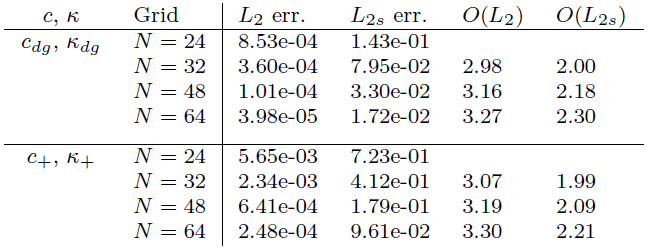
\includegraphics[height=35mm]{table_917} \\
%\caption{Accuracy of ESFR schemes for flow generated by a time-dependent source term on triangular grids, for the case of $p = 2$. The inviscid and viscous numerical fluxes were computed using a Rusanov flux with $\lambda = 1$ and a LDG flux with $\tau = 0.1$ and $\beta = \pm 0.5n$.}
%\label{fig:table_917}
%\end{figure}
%
%\begin{figure}
%\centering
%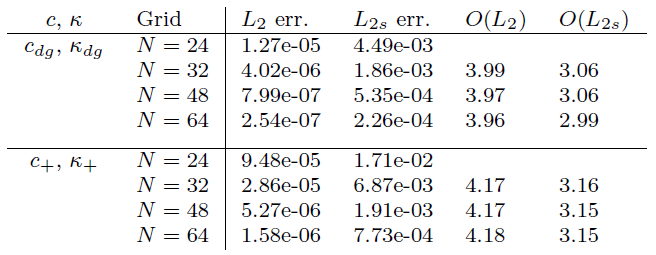
\includegraphics[height=35mm]{table_918} \\
%\caption{Accuracy of ESFR schemes for flow generated by a time-dependent source term on triangular grids, for the case of $p = 3$. The inviscid and viscous numerical fluxes were computed using a Rusanov flux with $\lambda = 1$ and a LDG flux with $\tau = 0.1$ and $\beta = \pm 0.5n$.}
%\label{fig:table_918}
%\end{figure}
%
%\begin{figure}
%\centering
%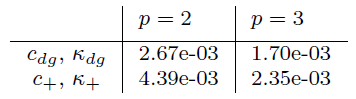
\includegraphics[height=20mm]{table_919} \\
%\caption{Explicit time-step limits ($\Delta t_{max}$) of ESFR schemes for flow generated by a time-dependent source term on the triangular grid with $\tilde{N} = 48$, for the cases of $p = 2$ and $3$. The inviscid and viscous numerical fluxes were computed using a Rusanov flux with $\lambda = 1$ and a LDG flux with $\tau = 0.1$ and $\beta = \pm 0.5n$.}
%\label{fig:table_919}
%\end{figure}
%
%\begin{figure}
%\centering
%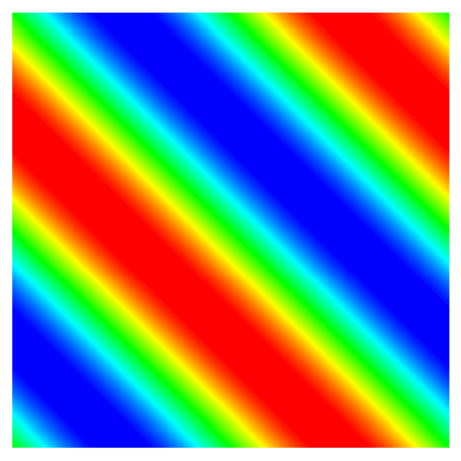
\includegraphics[height=60mm]{figure_912} \\
%\caption{Contours of energy obtained using the ESFR scheme with $c = c_+$ and $\kappa = \kappa_+$ on the triangular grid with $\tilde{N} = 32$ for the case of $p = 3$. The inviscid and viscous numerical fluxes were computed using a Rusanov flux with $\lambda = 1$ and a LDG flux with $\tau = 0.1$ and $\beta = \pm 0.5n$.}
%\label{fig:figure_912}
%\end{figure}
%
%\begin{figure}
%\centering
%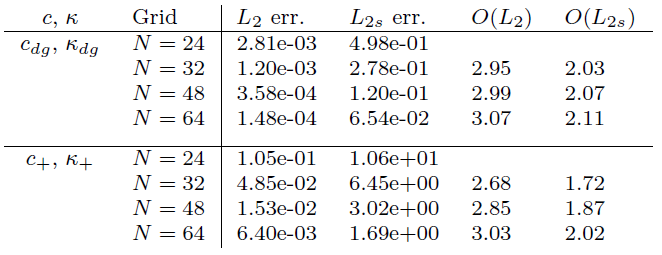
\includegraphics[height=35mm]{table_920} \\
%\caption{Accuracy of ESFR schemes for flow generated by a time-dependent source term on tetrahedral grids, for the case of $p = 2$. The inviscid and viscous numerical fluxes were computed using a Rusanov flux with $\lambda = 1$ and a LDG flux with $\tau = 0.1$ and $\beta = \pm 0.5n$.}
%\label{fig:table_920}
%\end{figure}
%
%\begin{figure}
%\centering
%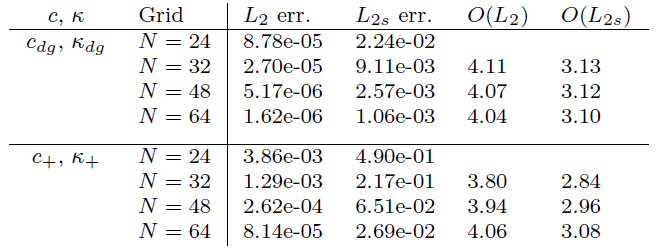
\includegraphics[height=30mm]{table_921} \\
%\caption{Accuracy of ESFR schemes for flow generated by a time-dependent source term on tetrahedral grids, for the case of $p = 3$. The inviscid and viscous numerical fluxes were computed using a Rusanov flux with $\lambda = 1$ and a LDG flux with $\tau = 0.1$ and $\beta = \pm 0.5n$.}
%\label{fig:table_921}
%\end{figure}
%
%\begin{figure}
%\centering
%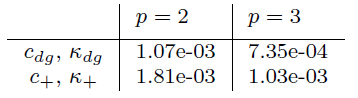
\includegraphics[height=15mm]{table_922} \\
%\caption{Explicit time-step limits ($\Delta t_{max}$) of ESFR schemes for flow generated by a time-dependent source term on the triangular grid with $\tilde{N} = 48$, for the cases of $p = 2 and 3$. The inviscid and viscous numerical fluxes were computed using a Rusanov flux with $\lambda = 1$ and a LDG flux with $\tau = 0.1$ and $\beta = \pm 0.5n$.}
%\label{fig:table_922}
%\end{figure}
%
%\newpage
%\begin{figure}
%\centering
%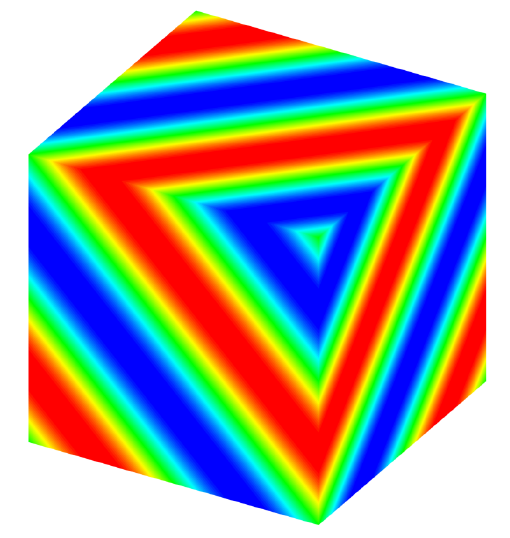
\includegraphics[height=60mm]{figure_913} \\
%\caption{Contours of energy obtained using the ESFR scheme with $c = c_+$ and $\kappa = \kappa_+$ on the tetrahedral grid with $\tilde{N} = 32$ for the case of $p = 3$. The inviscid and viscous numerical fluxes were computed using a Rusanov flux with $\lambda = 1$ and a LDG flux with $\tau = 0.1$ and $\beta = \pm 0.5n$.}
%\label{fig:figure_913}
%\end{figure}
